\newpage
\section{Auswertung}
\label{sec:auswertung}
\subsection{Eigenschaften des Röntgenstrahls}
    \begin{figure}[ht]
        \centering
        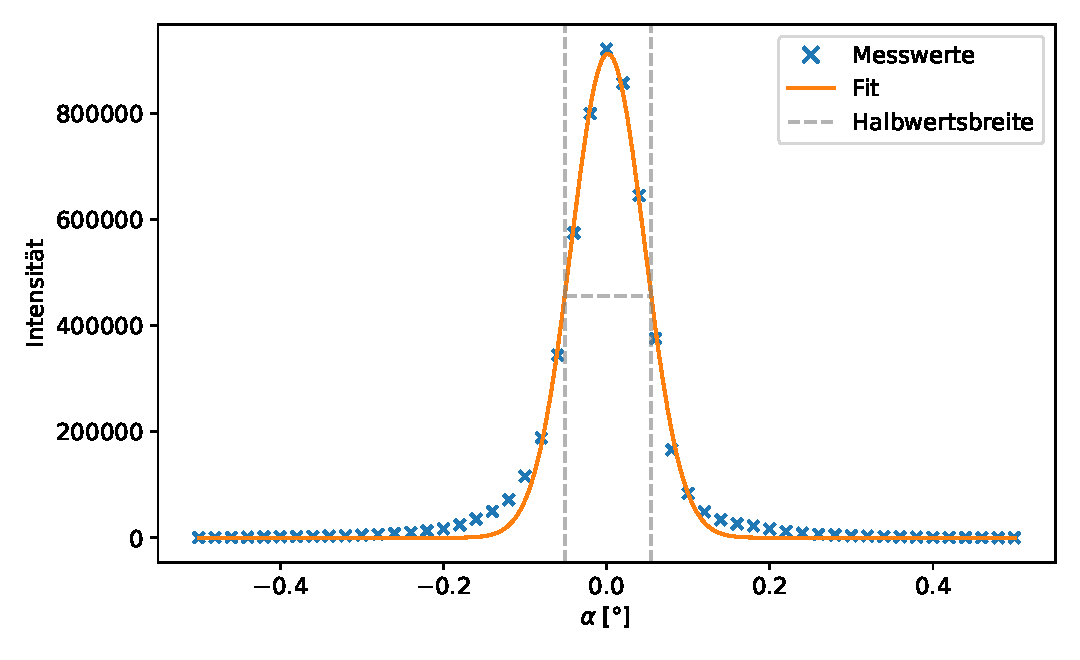
\includegraphics[width = 0.9\textwidth]{plots/DetektorScan.pdf}
        \caption{An die mit dem Detektorscan im Winkelbereich $0,5°$ bis $0,5°$ mit einer Schrittweite von $0,02°$ aufgenommenen Messwerte wird eine Gaußfunktion gefittet.}
        \label{fig:DetektorScan}
    \end{figure}

    Im Detektorscan werden die Intensitäten bei verschiedenen Winkel des Detektors zur Probe aufgenommen.
    Es ergibt sich eine gaußähnliche Intensitätsverteilung an die eine Gaußfunktion der Form
    \begin{equation*}
        f(\alpha) = A \cdot \exp\left(- \frac{(\alpha - \alpha_0)^2}{2 c^2}\right)
    \end{equation*}
    fitten lässt mit den Parametern
    \begin{align*}
        A &= 913152 \pm 10600 \\
        \alpha_0 &= 0,0016° \pm 0,0006° \\
        c &= 0,0449° \pm 0,0006° \,,
    \end{align*}
    wobei $A$ die Höhe des Peaks, $\alpha_0$ die Position des Peaks und $c$ die Standardabweichung ist.
    Mit diesen Anpassung werden die beiden wichtigsten Eigenschaften des Röntgenstrahls bestimmt, zum einen die Halbwertsbreite (FWHM) der Verteilung, zum anderen die maximale Intensität $I_0$ des Strahls.
    \begin{align*}
        \mathrm{FWHM} &= 2 c \sqrt{\ln(4)} = 0,1058° \pm 0,0014° \\
        I_0 &= A = 913152 \pm 10600 \,.
    \end{align*}

\newpage
\subsection{Bestimmung des Geometriewinkels}
\label{sec:BestimmungGeometriewinkel}
    Der Geometriewinkel kennzeichnet die Grenze ab der kleinere Winkel zwischen Strahl und Probe dazu führen würden, dass der Strahl eine größere Fläche überstreicht als die Probenoberfläche. \\
    Es gibt zwei Arten wie dieser Winkel mit den hier durchgeführten Messungen bestimmt werden kann.

    \begin{figure}[ht]
        \centering
        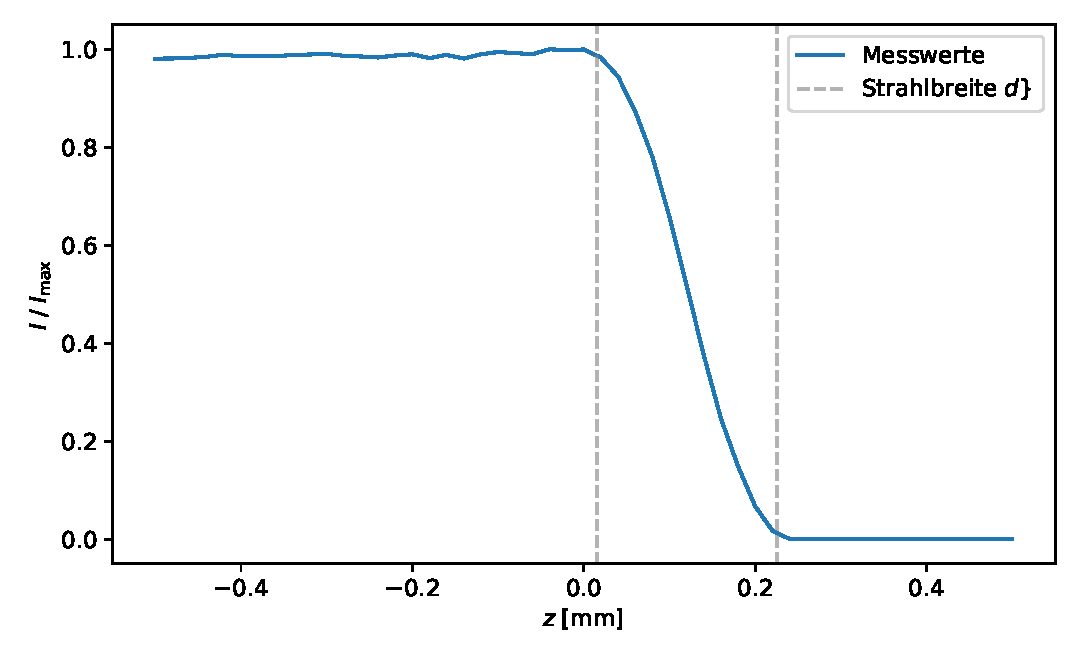
\includegraphics[width = 0.8\textwidth]{plots/Strahlbreite.pdf}
        \caption{Aus dem Graphen des zweiten Z-Scans bei $2\theta = 0°$ wird die Strahlbreite des Röntgenstrahls abgelesen.}
        \label{fig:Strahlbreite}
    \end{figure}
    Die Breite der fallenden Flanke im Graphen des ersten oder zweiten Z-Scans, wie in \autoref{fig:Strahlbreite} zu sehen, entspricht der Strahlbreite des Röntgenstrahls.
    Hier wurde der zweite Z-Scan gewählt vor dem Hintergrund, dass der Strahl nach dem ersten Rockingscan ausreichend parallel zur Probe verläuft und so die Strahlbreite genauer abzulesen ist.
    Praktisch ist die Probe schon vor dem Rockingscan parallel genug zum Strahl, sodass die abgelesenen Strahlbreiten bei dem ersten und zweiten Z-Scan gleich sind. \\
    Mithilfe der Kenntnis der Strahlbreite $d_0 = \SI{0,21}{mm}$ und der Probenlänge $D = \SI{20}{mm}$ wird nun der Geometriewinkel bestimmt:
    \begin{equation*}
        \alpha_{\mathrm{geo,z}} = \arcsin\left(\frac{d_0}{D}\right) \approx 0,6016°
    \end{equation*}
    
    \begin{figure}[ht]
        \centering
        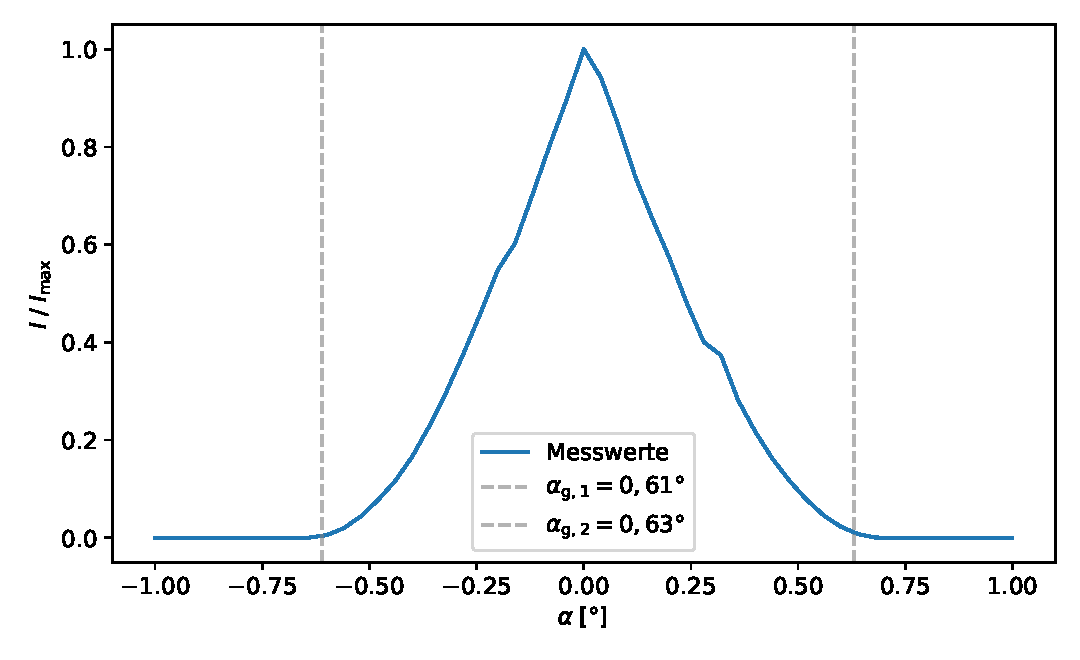
\includegraphics[width = 0.7\textwidth]{plots/Geometriewinkel.pdf}
        \caption{Aus dem Graphen des ersten RockingScans bei $2\theta = 0°$ wird der Geometriewinkel an dem Anfangspunkt der steigenden und dem Endpunkt der fallenden Flanke abgelesen.}
        \label{fig:Geometriewinkel}
    \end{figure}
    Es ist auch möglich den Geometriewinkel direkt aus dem Graphen des ersten Rockingscans in \autoref{fig:Geometriewinkel} auszulesen. Dabei ergeben sich zwei Winkel über die gemittelt wird:
    \begin{equation*}
        \alpha_{\mathrm{geo,rock}} = \frac{\alpha_{\mathrm{geo,1}} + \alpha_{\mathrm{geo,2}}}{2} = 0,62°
    \end{equation*}

    Wird der bestimmte Geometriewinkel unterschritten, so wird die einfallende Intensität mit dem Geometriefaktor, welcher das Verhältnis der Strahlbreite, die die Probe trifft und der Gesamtstrahlbreite darstellt, multipliziert und somit korrigiert.

\subsection{Reflektivitätskurve}
    Die erste Messung der Reflektivität enthält auch unerwünschte Anteile aus gestreuten Intensitäten.
    Um die Messwerte des Reflektivitätsscans zu korrigieren werden die Messwerte des Diffuser Scans von ihnen abgezogen.
    Dabei sind beide Messungen identisch bis auf das Verschieben des Detektorwinkels beim Diffuser Scan um 0,1° gegenüber dem Einfallswinkel, sodass dabei überwiegend Streuungen gemessen werden.
    \begin{equation*}
        R_{\mathrm{exp}} = \frac{I - I_{\mathrm{diff}}}{5 \cdot I_0}
    \end{equation*}
    Die Differenz wird auf die im zweiten Z-Scan bestimmte Intensität des einfallenden Strahls $I_0$ normiert. Da die Reflektivitätsmessung je Messwert 5s dauerte und der die Messdauer pro Messwert beim Z-Scan 1s betrug, wird durch $5 \cdot I_0$ geteilt.

    Zum Vergleich wird außerdem die Fresnelreflektivität einer ideal glatten Siliziumschicht nach \autoref{eqn:fresnel} in \autoref{fig:Reflektivitaetskurve1} eingezeichnet. Dazu werden die folgenden Daten aus \cite{tu_dortmund_versuchsanleitung_2021_e1} entnommen:
    \begin{enumerate}
        \setlength{\itemindent}{70pt}
        \item[Grenzwinkel:] $\quad \alpha_c \approx \sqrt{2 \delta} = \sqrt{2 \cdot 7,6 \cdot 10^{-6}} \approx 0,223°$
        \item[Wellenänge:] $\quad \lambda = 1,54 \cdot 10^{10} \;$m 
        \item[Absorption:] $\quad \beta = \frac{\lambda}{4 \pi} \mu = \frac{1,54 \cdot 10^{10} \; \mathrm{m}}{4 \pi} \cdot 141 \cdot 10^2 \; \frac{1}{\mathrm{m}} \approx 1,73 \cdot 10^{-7}$ 
    \end{enumerate}
    \begin{figure}[ht]
        \centering
        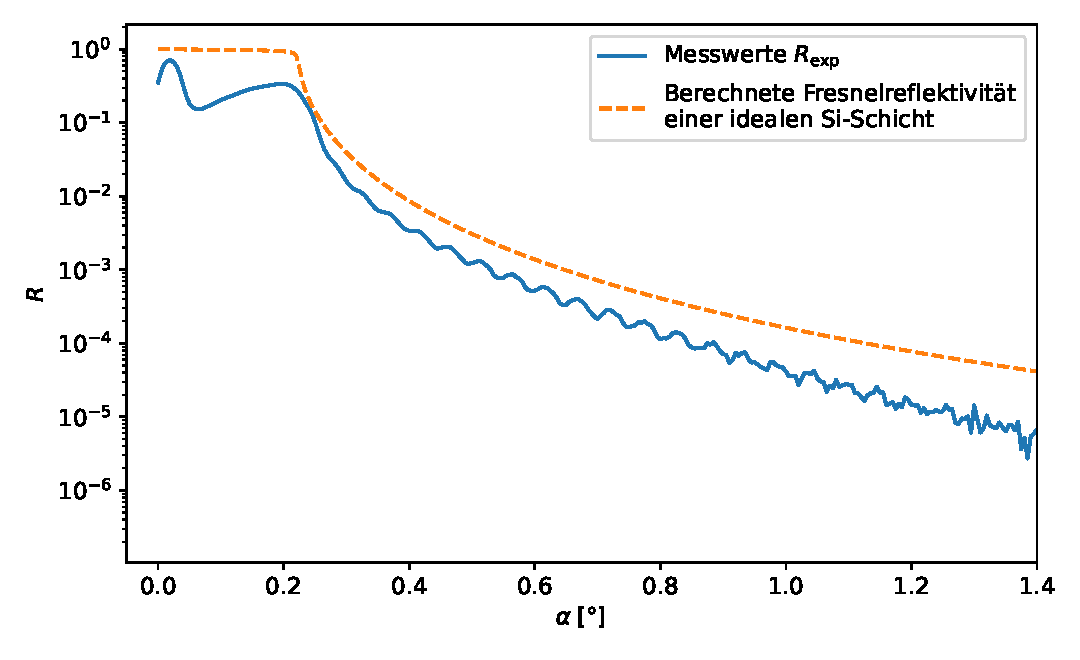
\includegraphics[width = 0.8\textwidth]{plots/Reflektivitaetskurve1.pdf}
        \caption{Von den aufgenommenen Messwerten der Reflektivität der Probe im Bereich 0° bis 2,5° werden die Messwerte der Reflektivität des \glqq Diffuser Scans\grqq{} im gleichen Messbereich abgezogen und hier dargestellt. Die berechnete Fresnel-Reflektivität für eine ideal glatte Siliziumschicht sind hier in orange zu dargestellt.}
        \label{fig:Reflektivitaetskurve1}
    \end{figure}

    Im Anschluss daran wird die in \autoref{fig:Reflektivitaetskurve1} gezeigte Reflektivitätskurve um den zuvor in \autoref{sec:BestimmungGeometriewinkel} bestimmten Geometriefaktor korrigiert falls der Geometriewinkel $\alpha_{\mathrm{geo}}$ unterschritten wird. Die korrigierte Reflektivität ergibt sich also zu
    \begin{equation*}
        R_{\mathrm{exp, korr}} =
        \begin{cases}
            \frac{R_{\mathrm{exp}}}{G} & \mathrm{bei} \quad \alpha < \alpha_{\mathrm{geo}} \\[3pt]
            \hspace{7pt} 1 & \mathrm{bei} \quad \alpha > \alpha_{\mathrm{geo}}
        \end{cases}
    \end{equation*}

    Die Schichtdicke kann nun auf zwei Arten bestimmt werden.
    Zur Abschätzung werden die Abstände zwischen den in \autoref{fig:Reflektivitaetskurve2} eingezeichneten Maxima verwendet.
    Es wird über alle Abstände gemittelt
    \begin{equation*}
        \overline{\varDelta \alpha} = (0,0532 \pm 0,0015)°
    \end{equation*}
    und somit ergibt sich eine Schichtdicke von
    \begin{equation*}
        d = \frac{\lambda}{2 \overline{\Delta \alpha}} = (830 \pm 24) \; \text{\AA} \;.
    \end{equation*}

    Bei der zweiten Methode wird der rekursive Parratt-Algorithmus \ref{eqn:parratt} für ein Zwei-Schicht-System, bestehend aus einer dünnen Schicht Polysterol und dem Substrat Silizium, verwendet. Alle für die Rechnung benötigten Daten wurden aus \cite{tu_dortmund_versuchsanleitung_2021_e1} entnommen.
    Die Fresnelkoeffizienten werden nach \autoref{eqn:rauheit} an die Rauheit der Grenzflächen angepasst.
    Die freien Parameter der Polysterol-Schichtdicke $d$, der Dispersionen von Polysterol $\delta_2$ und Silizium $\delta_3$, der Rauheiten der Grenzflächen $\sigma_1$ und $\sigma_2$ werden nun händisch angepasst.
    Zuerst wird die Schichtdicke auf den zuvor berechneten Wert gesetzt und die Dispersionen werden variiert, sodass die Werte der Theoriekurve möglichst nah an den gemessenen Werte liegen.
    Im Anschluss wird über die Schichtdicke der Abstand zwischen den Extrema eingestellt und die Rauheiten werden so angepasst, dass die gemessene und die theoretische Kurve auch bei größeren Winkeln möglichst gut übereinender liegen.

    Die so erhaltenen Parameter sind im Folgenden angegeben:
    \begin{align*}
        d_{\mathrm{p}} &= 860 \; \text{\AA} \\
        \delta_2 &= 1,0 \cdot 10^{-6} \\
        \delta_3 &= 7,0 \cdot 10^{-6} \\
        \sigma_1 &= 8,0 \cdot 10^{-10} \frac{1}{\text{\AA}}\\
        \sigma_2 &= 6,8 \cdot 10^{-10} \frac{1}{\text{\AA}}\\
    \end{align*}
    
    \begin{figure}[ht]
        \centering
        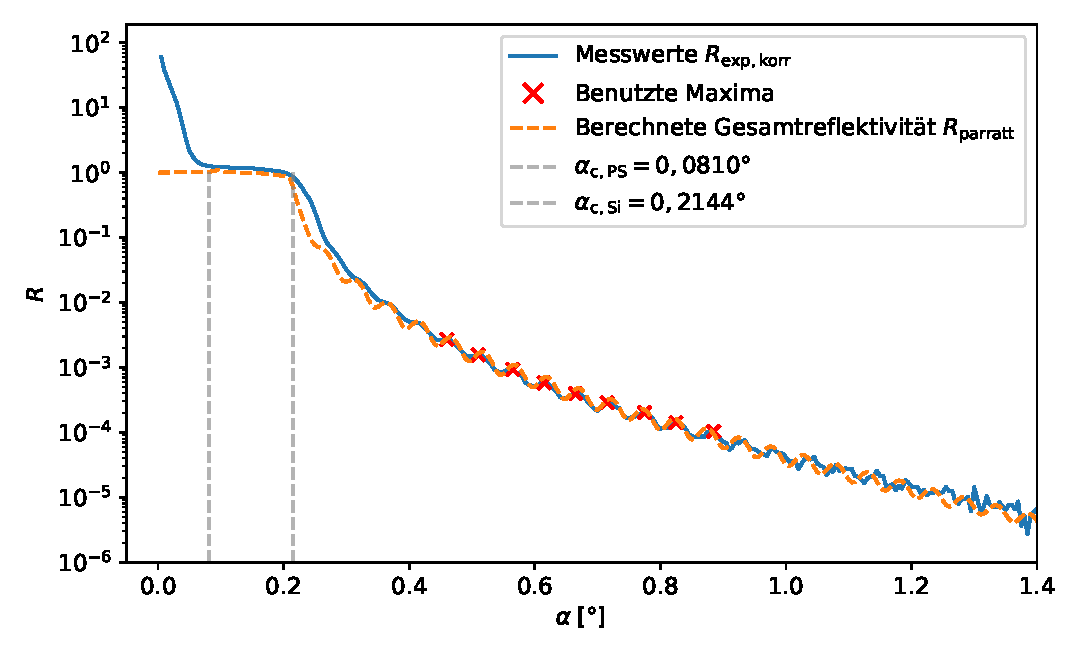
\includegraphics[width = 0.9\textwidth]{plots/Reflektivitaetskurve2.pdf}
        \caption{Die um den Geometriefaktor korrigierten Messwerte der Reflektivität sind hier dargestellt. Die gestrichelte Kurve wurde mithilfe des Parratt-Algorithmus für raue Grenzflächen an die Messwerte angepasst.}
        \label{fig:Reflektivitaetskurve2}
    \end{figure}

    Zum Schluss werden, mit den aus der Anpassung ermittelten Werten für die Dispersionen, die kritischen Winkel für Polysterol und Silizium ermittelt anhand von $\alpha_{\mathrm{c,}i} \approx \sqrt{2 \delta_i}$.
    \begin{align*}
        \alpha_{\mathrm{c,PS}} \approx \sqrt{2 \delta_2} = 0,0810° \\
        \alpha_{\mathrm{c,Si}} \approx \sqrt{2 \delta_3} = 0,2144°
    \end{align*}